
\documentclass[10pt, openany]{book}

%PACKAGES%

\usepackage[inner=0.75in, outer=0.75in, top=0.75in, bottom=0.75in, a5paper]{geometry}
\usepackage{graphicx}
\usepackage{fontspec, newunicodechar}
%\usepackage{sectsty}
\usepackage{titlesec}
\usepackage{verse}
\usepackage[unicode, pdfauthor={Bhikkhu Sunyo}, pdftitle={Viññāṇa Anidassana: The state of boundless consciousness}, pdfsubject={Buddhism}, pdfkeywords={Buddhism}, pdfcreator={Wiswo-texBuilder}, hyperfootnotes=false]{hyperref} 

%links and cites
\hypersetup{
    colorlinks = true,
    linkcolor = [rgb]{0.1, 0.1, 0.56},
    anchorcolor = blue,
    citecolor = blue,
    filecolor = blue,
    urlcolor = [rgb]{0.4, 0.6, 0.91}
    }

%MICROTYPOGRAPHY%
\usepackage{microtype}

\hyphenpenalty=750


\usepackage{enumitem}
\setlist[itemize]{labelsep=1em, leftmargin=10mm}

%LINESPACE%
\usepackage{setspace}
\setstretch{1.20}
\setlength{\parskip}{0pt}

%Minimum space before footnotes
\setlength{\skip\footins}{1\baselineskip}
\setlength{\footnotesep}{11pt}

%VERSE%
\settowidth{\versewidth}
{mmmmmmmmmmmmmmmmmmm}%THIS SETS THE GLOBAL DEFAULT WIDTH OF CENTERING. IT IS USUALLY DETERMINED LOCALLY, HOWEVER.%
%VERSE%


%HEADER%
\usepackage{fancyhdr}
\setlength{\headheight}{15pt}
\pagestyle{fancy}

\fancyhf{}
%\fancyfoot[CE,CO]{– \thepage \hspace{0.18em}–}

\fancyhead[RO]{\headerfont\scshape\small\textcolor[rgb]{0.5, 0.5, 0.5}{Viññāṇa Anidassana —\hspace{0.18em}\thepage}}
\fancyhead[LE]{\headerfont\scshape\small\textcolor[rgb]{0.5, 0.5, 0.5}{\thepage\hspace{0.18em}— Bhikkhu Sunyo}}

\renewcommand{\headrulewidth}{0pt}
\fancypagestyle{plain}{ %
\fancyhf{} % remove everything
\renewcommand{\headrulewidth}{0pt}
\renewcommand{\footrulewidth}{0pt}
}

\renewcommand\footnoterule{{\color[rgb]{0.8, 0.8, 0.8} \hrule width 1in height 0.2pt}} % a 1 inch gray line 


%FONTS%
\setmainfont[]{Gentium Book Plus}
\setsansfont[]{Linux Biolinum O}
%FONTS%

\titleformat{\chapter}
{\center\Huge\Chapfont\scshape}
{}
{0pt}
{}

\titleformat{\section}
{\vspace{4pt}\linespread{1}\center\Large\scshape\Secfont}
{}
{0pt}
{}

\setcounter{secnumdepth}{-1}

\newfontfamily\Chapfont[]{Wiswo Small Caps}
%\newfontfamily\Chapnumfont{Source Sans 3}
\newfontfamily\Secfont[]{Wiswo Small Caps}
%\sectionfont{\linespread{0.75}\center\Large\Secfont}
\newfontfamily\headerfont[]{Wiswo Small Caps}

\newfontfamily\Titlefont[]{Wiswo Small Caps}

%EPIGRAPH%
\newenvironment{epigraph}


%HANGING LEFT%
\newcommand*{\vleftofline}[1]{\leavevmode\llap{#1}}

%WIDOWS & ORPHANS%
\widowpenalty=10000
\clubpenalty=10000

\counterwithout{footnote}{chapter}
\usepackage[hang,flushmargin,bottom]{footmisc}
%\graphicspath{ {./images/} }

\newcommand{\nocontentsline}[3]{}
\newcommand{\tocless}[2]{\bgroup\let\addcontentsline=\nocontentsline#1{#2}\egroup}

\makeatletter
\newcommand{\epubchapter}[1]{%
  \begingroup
  \let\@makechapterhead\@gobble % make \@makechapterhead do nothing
  \tocless \chapter{#1}
  \endgroup
}
\makeatother

\usepackage{verbatim}


\pretolerance=400
\tolerance=800
\emergencystretch=3pt

\newenvironment{aphorism}%
{%
\begin{center}\begin{itshape}
}%
{\end{itshape}\end{center}
}%

\hyphenation{manu-scripts}

\makeatletter
\def\@biblabel#1{}
\renewcommand\@cite[2]{{#1\if@tempswa,\nolinebreak[3] #2\fi}}
\makeatother

\makeatletter
\renewenvironment{thebibliography}[1]
     {\section{\bibname}% <-- this line was changed from \chapter* to \section
      \@mkboth{\MakeUppercase\bibname}{\MakeUppercase\bibname}%
      \list{\@biblabel{\@arabic\c@enumiv}}%
           {\settowidth\labelwidth{\@biblabel{#1}}%
            \leftmargin\labelwidth
            \advance\leftmargin\labelsep
            \@openbib@code
            \usecounter{enumiv}%
            \let\p@enumiv\@empty
            \renewcommand\theenumiv{\@arabic\c@enumiv}}%
      \sloppy
      \clubpenalty4000
      \@clubpenalty \clubpenalty
      \widowpenalty4000%
      \sfcode`\.\@m}
     {\def\@noitemerr
       {\@latex@warning{Empty `thebibliography' environment}}%
      \endlist}
\makeatother



\begin{document}

\frontmatter

\pagestyle{empty}

%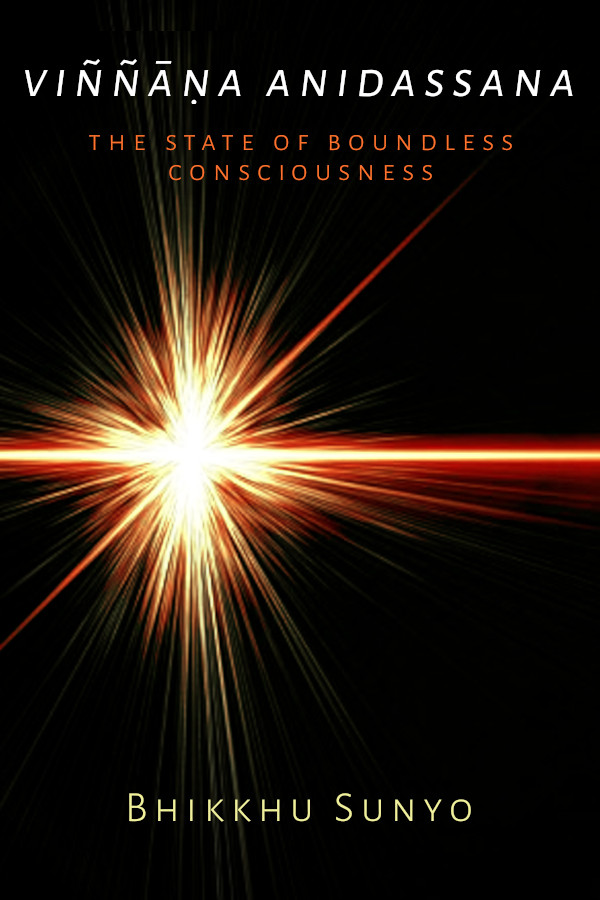
\includegraphics[scale= 2, trim= 0 0 0 0]{../_resources/book-data/vasy/FrontLarge.jpg}

\newpage~\newpage~

\begin{center}
\vspace{2em}

\Huge\Titlefont\scshape{Viññāṇa Anidassana}\\
\vspace{0.5em}
\large\Titlefont\scshape{The state of boundless consciousness}\\

\begin{Large}
\vspace{4em}
\Titlefont\scshape{Bhikkhu Sunyo}
\end{Large}


\vspace*{\fill}
%
\includegraphics[scale=0.06, trim = 0 13 5 0 ]{../_resources/images/icons/logo-enso-large}\\
\vspace{4pt}
\begin{small}
\scshape{Wisdom \& Wonders\\
Books}
\end{small}
\end{center}

\newpage
\begin{small}
\begin{sffamily}
\noindent Copyright © — Bhikkhu Sunyo\\

\noindent Originally published in 2021.\\\noindent This edition published in 2022.\\\noindent Addendum added 2024.\\

\noindent\textbf{CC0 1.0 Universal (CC0 1.0) Public Domain Dedication}\\



\noindent\textbf{No Copyright}

\noindent The person who associated a work with this deed has dedicated the work to the public domain by waiving all of his or her rights to the work worldwide under copyright law, including all related and neighboring rights, to the extent allowed by law.

\noindent You can copy, modify, distribute and perform the work, even for commercial purposes, all without asking permission. See Other Information below.


\noindent\textbf{Other Information}

\noindent In no way are the patent or trademark rights of any person affected by CC0, nor are the rights that other persons may have in the work or in how the work is used, such as publicity or privacy rights.

\noindent Unless expressly stated otherwise, the person who associated a work with this deed makes no warranties about the work, and disclaims liability for all uses of the work, to the fullest extent permitted by applicable law.

\noindent When using or citing the work, you should not imply endorsement by the author or the affirmer.

\end{sffamily}
\end{small}


\tableofcontents

\mainmatter
\pagestyle{fancy}

			
			
			

\chapter{Introduction}
A wide range of opinions has long surrounded two innocent Pali words: \textit{viññāṇa anidassana}. They are translated variously, as ‘consciousness that is without feature / signless / invisible / non-manifesting / makes no showing / can not be characterized’, et cetera. This variety already indicates that their meaning is somewhat obscure. This obscurity has, however, not stopped interpreters from giving the words a lot of importance, because some see in \textit{viññāṇa} \textit{anidassana} a kind of consciousness essentially equal to nibbāna.\footnote {The first to equate \textit{viññāṇa anidassana} to nibbāna is, to my knowledge, \cite{Falk} 1943. But this and similar ideas are still very alive today.} But there are many problems with this, starting with the following:


\begin{itemize}

\itemsep5pt\parskip0pt\parsep0pt


\item
No sutta equates nibbāna to any type of consciousness.



\item
Many suttas do the exact opposite: they relate nibbāna to the cessation of consciousness,\footnote {E.g. \href{https://suttacentral.net/sn1.2/en/sujato\#5.2}{SN 1.2:5.2}, \href{https://suttacentral.net/an3.90/en/sujato\#9.1}{AN 3.90:9.1–9.4}, \href{https://suttacentral.net/snp3.12/en/sujato\#18.3}{Snp 3.12:18.3–20.4}, \href{https://suttacentral.net/ud8.9/en/sujato\#5.4}{Ud 8.9:5.4}} and equate consciousness to suffering.\footnote {E.g.  \href{https://suttacentral.net/sn22.10/en/sujato\#1.10}{SN 22.10:1.10–1.11}}



\item
There are only two mentions of \textit{viññāṇa anidassana} in the Pali suttas, and other early suttas don’t have the concept at all. This makes the words not only difficult to interpret, but also unlikely to be a core teaching on such a central topic as nibbāna.





\end{itemize}
Some things are just best explained in writing—hence this essay. I show here that \textit{viññāṇa anidassana} is not nibbāna, but a poetic description of the state of boundless consciousness, the second “formless” meditation state. Most of the arguments were made before by others.\footnote {\cite{Anālayo 2017}, \cite{Brahmali}, \cite{Sujato 2011a}, and \cite{Sujato 2011b}, among others.} I gathered them here, together with a few thoughts of my own.


This essay analyzes rare terms in abstract texts. However, it also illustrates the nature of Pali verse, and provides a good example of how to apply the Buddha’s advice on deciding what his real teachings were.


For accessibility I have mostly adopted common translations for Pali words—such as ‘form’ for \textit{rūpa}—even though these may not be my personal preferences.


\chapter{1. The Kevaddha Sutta}
As stated, the suttas mention \textit{viññāṇa anidassana} twice: once in the Kevaddha (With Kevaddha) Sutta,\footnote {\href{https://suttacentral.net/dn11/en/sujato\#85.18}{DN 11:85.18}} and once in the Brahmanimantanika (Invitation of a Brahmā) Sutta.\footnote {\href{https://suttacentral.net/mn49/en/sujato\#25.1}{MN 49:25.1}} We will look at them separately.


In the Kevaddha Sutta the Buddha tells a layman named Kevaddha a story of an unnamed monk who ascends various heavens searching for an answer to a question. This monk’s strategy is, to put it mildly, somewhat unusual. Monks ordinarily brought their questions directly to the Buddha or one of his close disciples. The story seems to be symbolic, the monk’s astral travels being a metaphor for looking for enlightenment in the wrong place. The story probably parodies brahmin ideas, because the gods, including Brahmā, all failed to answer the monk’s question.


To put a long story short: After visiting higher and higher heavens while never finding an answer, the monk ends up asking Brahmā his question: “Where do the four elements—earth, water, fire, and air—cease without remnant?” He essentially wants to know where form (\textit{rūpa}) ceases, because according to the ideas of the time “all form of whatever kind is the four elements”.\footnote {\href{https://suttacentral.net/an11.17/en/sujato\#3.1}{AN 11.17:3.1–3.3}} Brahmā does not know the answer, so he sends the monk to the Buddha, who, when asked the same question, says it should be rephrased. He changes the question from “where do earth, water, fire, and air [i.e. form] cease without remnant?” to “where do earth, water, fire, and air\textit{ find no footing}?” (This change is quite significant, as we’ll see later.) The Buddha then also adds a second question, asking where not only \textit{rūpa}, but \textit{nāma} ceases too. (\textit{Nāma}, literally ‘name’, in this context means something like ‘personal characteristics’. It stands for the immaterial aspects of an individual being, excluding consciousness. I will leave it untranslated.)


The Buddha presents the two questions in a six-line verse, and then answers those questions in two separate verses:


\begin{quote}


\begin{itemize}

\item[{[Q1]}]“Where do earth, water, \\ fire, and air find no footing?


\item[{[Q2]}]Where do the long and short, \\ the small and gross, the fair and ugly— \\ where do \textit{nāma} and form \\ fully come to cease?

\end{itemize}

\end{quote}
For that the explanation is:


\begin{quote}


\begin{itemize}

\item[{[A1]}]Boundless consciousness, \\ invisible, fully shining: \\ here earth, water, \\ fire, and air find no footing.


\item[{[A2]}]Here the long and short, \\ the small and gross, the fair and ugly— \\ here \textit{nāma} and form \\ fully come to cease: \\ when consciousness ceases, \\ then those come to cease.”\footnote {\href{https://suttacentral.net/dn11/en/sujato\#85.11}{DN 11:85.11–85.27} [PTS: D I 223] ‘\textit{Kattha āpo ca pathavī, tejo vāyo na gādhati? Kattha dīghañca rassañca, aṇuṁ thūlaṁ subhāsubhaṁ; Kattha nāmañca rūpañca, asesaṁ uparujjhatī’ti? Tatra veyyākaraṇaṁ bhavati: ‘Viññāṇaṁ anidassanaṁ, anantaṁ sabbato pabhaṁ; Ettha āpo ca pathavī, tejo vāyo na gādhati. Ettha dīghañca rassañca, aṇuṁ thūlaṁ subhāsubhaṁ; Ettha nāmañca rūpañca, asesaṁ uparujjhati; Viññāṇassa nirodhena, etthetaṁ uparujjhatī’ti}.}

\end{itemize}

\end{quote}
(A similar structure of multiple questions and answers exists in the Sutta Nipata.)\footnote {\href{https://suttacentral.net/snp4.11/en/sujato}{Snp 4.11}}


\vspace* {1em}\noindent
But now comes the crux of the matter. Some interpret the two answer verses to contain one single answer—somewhat like this:


\begin{quote}


\begin{itemize}

\item[{[A]}]“Boundless consciousness, \\ invisible, fully shining: \\ here earth, water, \\ fire, and air find no footing, \\ here the long and short, \\ the small and gross, the fair and ugly— \\ here \textit{nāma} and form \\ fully come to cease: \\ when consciousness ceases, \\ then those come to cease.”

\end{itemize}

\end{quote}
This tiny change in punctuation—removing a period—turns it all into quite a riddle. Boundless consciousness now seems to be equal to the cessation of \textit{nāma} and form, and therefore (if we also ignore the last two lines) to nibbāna.


The underlying problem is that the original Pali manuscripts do not have punctuation such as periods and question marks. Translators have to add these themselves, and it is not always obvious where to do so. In this case the various lines starting with the word ‘here’ can easily confuse. It may even be that the transition between the two answers is somewhat vague on purpose. The Buddha could be saying something like: “I got a lot of money … stolen from me!” The meaning only becomes clear when you come to the end, to the cessation of consciousness. This is a poetical device if anything, and we are talking about poems here.


Either way, there are various more concrete reasons to divide the answer verses into two:


\begin{itemize}

\itemsep5pt\parskip0pt\parsep0pt


\item
All translators seem to recognize there are two sentences in the question verse, because it has two main verbs: ‘find a footing’ and ‘come to cease’. But many seem to miss that these two verbs ask very different things. ‘To find no footing’ means something very different than ‘to cease’. This is exactly why the Buddha made the change in the monk’s original question! So, there being two distinct questions, there should be two distinct answers too.



\item
The first answer ends with a main verb (\textit{gādhati} ‘find footing’), which in Pali commonly indicates the end of a sentence.



\item
Sentences only rarely run from one verse to the next.



\item
The first answer verse mentions the existence of a type of consciousness (boundless consciousness), the second the cessation of consciousness. These opposites are not both part of the same answer.



\item
Most importantly, when seen as two separate answers, the verses become standard teachings found throughout the suttas, not unique ones found only here (which they would be if \textit{viññāṇa anidassana} were nibbāna).





\end{itemize}
The rest of this section clarifies this last statement in detail. But first it is important to emphasize that the questions and answers are all \textit{verse}. Pali verse always needs to fit a certain pattern called ‘meter’. To be able to comply to this meter, verses are very free in their use of words. They often depart from convention or even literal accuracy, using what is known as poetic licence. In the analysis of verse these matters should always be taken into account.




\section{The first question}
Let me isolate the first question and answer:


\begin{quote}


\begin{itemize}

\item[{[Q1]}]“Where do earth, water, \\ fire, and air find no footing?”


\item[{[A1]}]“Boundless consciousness, \\ invisible, fully shining: \\ here earth, water, \\ fire, and air find no footing.”

\end{itemize}

\end{quote}
Remember, the question essentially asks, “where does \textit{form} find no footing?” The answer—“boundless consciousness, invisible, fully shining”—refers to the state of boundless consciousness, the second so-called formless state of meditation, also known as ‘the base of infinite consciousness’, or sometimes called ‘the sixth jhāna’. This is evident from the words ‘boundless’ (\textit{ananta}) and ‘consciousness’ (\textit{viññāṇa}). Not only do these make up the very name of the state of boundless consciousness, they also describe its attainment in the common formula, “focusing on ‘boundless consciousness’, one attains the state of boundless consciousness.”\footnote {E.g. \href{https://suttacentral.net/sn28.6/en/sujato\#1.3}{SN 28.6:1.3}: ‘\textit{anantaṁ viññāṇan’ti viññāṇañcāyatanaṁ upasampajja viharāti}.} The state of boundless consciousness is the only context in the suttas which uses the words ‘boundless’ and ‘consciousness’ together. It also occurs very frequently, so we should naturally assume the Buddha is referring to it here. Otherwise, if he would for example refer to nibbāna, he introduces here a teaching which is totally unique, in obscure verse, in just five words, out of which two would be easily mistaken as something else (namely the state of boundless consciousness).


In Pali the five words making up the answer are:


\begin{quote}


\begin{itemize}

\textit{viññāṇaṁ anidassanaṁ} (consciousness invisible) \\ \textit{anantaṁ sabbato pabhaṁ} (boundless fully shining)

\end{itemize}

\end{quote}
These words seem to be forced into their particular order by the meter of the verse, which requires eight syllables in each line. As A.K. Warder, a leading scholar of Pali verse, wrote: “Poetic licence is most noticeable in the freedom of word order in verse.”\footnote {\cite{Warder}} This means ‘boundless’ can be taken as the central adjective describing ‘consciousness’, with ‘invisible’ and ‘fully shining’ being secondary to it. That is to say, the latter two apply not to ‘consciousness’, but to ‘boundless consciousness’ as a whole. It is not consciousness that is fully shining and invisible, it is \textit{boundless consciousness} that is. I rearranged the words in my translation to clarify this. (Such rearrangement, let it be clear, is done often in translations of Pali.)


The term ‘fully shining’ (\textit{sabbato pabhaṁ}) is a metaphor, of course. The state of boundless consciousness does not literally give off light. It refers to the absence of the five mental hindrances in deep meditation. As the Upakkilesa (Impurities) Sutta in the Aṅguttara Nikāya says: “when the mind is freed from these five impurities [i.e. hindrances] it is \textit{shining}.”\footnote {\href{https://suttacentral.net/an5.23/en/sujato\#2.1}{AN 5.23:2.1–2.6}: \textit{Yato ca kho, bhikkhave, cittaṁ imehi pañcahi upakkilesehi vimuttaṁ hoti […] pabhassarañca}.} The suttas often compare a mind in deep meditation to something that gives off light, most commonly a fire.\footnote {E.g. \href{https://suttacentral.net/mn140/en/sujato\#20.1}{MN 140:20.1–20.3} [PTS: M III 243], \href{https://suttacentral.net/sn51.22/en/sujato\#3.1}{SN 51.22:3.1–4.3}, \href{https://suttacentral.net/an3.102/en/sujato\#1.6}{AN 3.102:1.6, 3.6}, \href{https://suttacentral.net/thag20.1/en/sujato\#59.1}{Thag 20.1:59.1–61.4}, \href{https://suttacentral.net/dhp387/en/sujato}{Dhp 387}}


Aside from the hindrances, another thing that is notably absent in the state of boundless consciousness is perceptions pertaining to ‘form’\footnote {E.g. \href{https://suttacentral.net/an9.31/en/sujato\#1.7}{AN 9.31:1.7–1.8}: “For one who has attained the base of boundless space, the perception of form has ceased. For one who has attained the base of boundless consciousness, the perception present in the base of boundless space has ceased.”. C.f. \href{https://suttacentral.net/an10.6/en/sujato}{AN 10.6} where in a list of (gradual) cessation of perception the formless attainments follows the four elements, i.e. form.} (which I understand to be a subtle mental perception, not a perception of the body). This is addressed by \textit{anidassana}, translated here quite literally as ‘invisible’. Since the meaning of \textit{rūpa} includes ‘appearance’,\footnote {Cf. e.g. Rhys Davids, \cite{PED}: “\textit{Rūpa}: form, figure, appearance, principle of form, etc.”} \textit{arūpa} means ‘without appearance’, thus ‘invisible’. This translation is in accordance with the apparent meaning of \textit{anidassana} in the Saṅgīti Sutta, which mentions visible form and invisible form (i.e. material form and the more subtle types such as in meditation).\footnote {\href{https://suttacentral.net/dn33/en/sujato\#1.10.75}{DN 33:1.10.75–1.10.76} [PTS: D III 217] \textit{Tividhena rūpasaṅgaho: sanidassanasappaṭighaṁ rūpaṁ, anidassanasappaṭighaṁ rūpaṁ, anidassanāppaṭighaṁ rūpaṁ}, “The threefold classification of form: visible tangible form, invisible tangible form, and invisible intangible form.”} The only other text that gives a useful context for \textit{anidassana} is the Kakacūpama Sutta, which says one can not paint the sky because “the sky is without form, invisible” (\textit{ākāso arūpī anidassano}).\footnote {\href{https://suttacentral.net/mn21/en/sujato\#14.1}{MN 21:14.1–14.10}} Here we see \textit{anidassana} indeed as a synonym of \textit{arūpa}.\footnote {Cf. \cite{Anālayo 2017} p.13: “This [\textit{anidassana}] also occurs in a description of space, which is said to be immaterial, \textit{arūpa}, and invisible, \textit{anidassana}, a context where the two terms seem to function as near synonyms.”}


We should not need to look for a deeper meaning behind \textit{anidassana}, because, as accurately stated by \cite{Warder} again, in verse “the need to fit the sentence to the meter influences the choice of vocabulary, so that unusual synonyms and rare words may be used.”\footnote {\cite{Warder} p.354} \textit{Anidassanaṁ} fits this perfectly: it is a rare and unusual synonym which supplies the meter \textit{arūpaṁ} and \textit{anantaṁ} could not. In summary, all it does is metaphorically describe the absence of form in the state of boundless consciousness, the second formless state.


Let's return to the question, “where does form find no footing?” Why is the answer the second formless state and not the first? This is because form can still “find a footing” in the first formless state, the state of boundless space. According to Sariputta in the Nibbānasukha Sutta, a perception pertaining to form can infiltrate this state and bring the mind back to the fourth jhāna: “After the complete transcendence of perceptions of forms, […] focusing on boundless space, a monk attains the state of boundless space. If in that state he begins to perceive or focus back on forms, that will be an affliction to him.”\footnote {\href{https://suttacentral.net/an9.34/en/sujato\#6.1}{AN 9.34:6.1–6.2}} The state of boundless consciousness is the lowest meditative state which can not be directly disturbed by such perceptions, and therefore it is “where form finds no footing”.


The state of boundless consciousness is still just a temporary escape from form, however, which explains why the Buddha changed the monk's question from “where do earth, water, fire, and air [i.e. form] \textit{cease without remnant}?”, which implies permanent cessation, to “where do earth, water, fire, and air \textit{find no footing}?”, which only implies a temporary inability to infiltrate. This change in the question can not be explained if the boundless consciousness of the Kevaddha Sutta were to be a permanent escape from form, like nibbāna.


As a sidenote, two other Pali suttas contain verses with the phrase “where earth, water, fire, and air find no footing”\footnote {\href{https://suttacentral.net/sn1.27/en/sujato\#2.1}{SN 1.27:2.1–2.2} \& \href{https://suttacentral.net/ud1.10/en/sujato\#14.1}{Ud 1.10:14.1–14.2}. The Chinese parallels of \href{https://suttacentral.net/sn1.27/en/sujato}{SN 1.27} (\href{https://suttacentral.net/sa601}{SĀ 601} and \href{https://suttacentral.net/sa-2.176}{SĀ-2 176}) appear not to have “where earth, water, fire, and air find no footing”. Cf. \cite{Sujato 2011b}.} and one has a similar line in an inspired utterance, which is technically prose, but is still very poetical.\footnote {\href{https://suttacentral.net/ud8.1/en/sujato\#3.1}{Ud 8.1:3.1–3.4}} These three suttas all refer to the cessation of the aggregates (\textit{khandhas}) after the death of an enlightened one, often called parinibbāna.\footnote {\href{https://suttacentral.net/sn1.27/en/sujato\#2.5}{SN 1.27:2.5–2.6} mentions the cessation of \textit{nāmarūpa}. In \href{https://suttacentral.net/ud1.10/en/sujato\#12.3}{Ud 1.10:12.3–15.4} the verses were spoken when monks asked about the faith of the arahant Bāhiya who just passed away. \href{https://suttacentral.net/ud8.1/en/sujato}{Ud 8.1} mentions the absence of all form and the formless. All other factors in this inspired utterance describe the end of rebirth from different perspectives. So all three texts are about nibbāna after death.} This does not pose any problems for the ideas laid out above, because form not only finds no footing in the state of boundless consciousness, but after parinibbāna finds no footing anywhere either. In other words: “where earth, water, fire, and air find no footing” is just a partial description of parinibbāna that also applies to the state of boundless consciousness. Just because it refers to parinibbāna in these suttas, does not mean it also does in the Kevaddha Sutta. A line of verse can describe one thing in one context, and another thing in another context. This is quite common in the suttas. An example is found right here in the Kevaddha Sutta. The line “the long and short, the small and gross, the fair and ugly”, which has such a deep meaning here, elsewhere simply refers to things one should not steal.\footnote {\href{https://suttacentral.net/mn98/en/sujato\#11.55}{MN 98:11.55–11.58} [PTS: M II 121] \& \href{https://suttacentral.net/dhp409/en/sujato}{Dhp 409}}




\section{The second question}
Here are the second question and answer again:


\begin{quote}


\begin{itemize}

\item[{[Q2]}]“Where do the long and short, \\ the small and gross, the fair and ugly— \\ where do \textit{nāma} and form \\ fully come to cease?”


\item[{[A2]}]“Here the long and short, \\ the small and gross, the fair and ugly— \\ here \textit{nāma} and form \\ fully come to cease: \\ when consciousness ceases, \\ then those come to cease.”

\end{itemize}

\end{quote}
Remember that this question was not originally asked by the monk, but was added by the Buddha. The Buddha did so to indicate the monk’s quest for the cessation of form did not reach far enough. The formless, included in \textit{nāma}, must cease as well.


The answer reflects a teaching found at least a hundred times elsewhere in the Pali Canon: “when consciousness ceases, \textit{nāma} and form will cease”—a stock phrase of Dependent Arising.\footnote {\textit{viññāṇanirodhā nāmarūpanirodho} in e.g. \href{https://suttacentral.net/sn12.1/en/sujato\#3.3}{SN 12.1:3.3}.} So here too, just as with the first question, the Buddha rephrases a teaching his audience would have been familiar with.


We find the same teaching in the Ajita’s Question Sutta in the Pārāyana Vagga:\footnote {\href{https://suttacentral.net/snp5.2/en/sujato\#6.3}{Snp 5.2:6.3–6.6}: \textit{yattha nāmañca rūpañca, asesaṁ uparujjhati; viññāṇassa nirodhena, etthetaṁ uparujjhati}.}


\begin{quote}


\begin{itemize}

\item[{}]“As to where \textit{nāma} and form \\ fully come to cease: \\ when consciousness ceases, \\ then those come to cease.”

\end{itemize}

\end{quote}
This verse is virtually identical to the Kevaddha Sutta. Yet the Ajita’s Question Sutta makes no mention of \textit{viññāṇa anidassana} or anything alike. The verse stands on its own as a complete teaching. This confirms that in the Kevaddha Sutta “where \textit{nāma} and form fully come to cease” is only connected to the cessation of consciousness, not to \textit{viññāṇa anidassana}.


Now nearing the end of Kevaddha Sutta, we can assume the astral-traveling monk of the story understood the Buddha’s teachings, since after the verses nothing else is asked. And after being told the story, Kevaddha also asks no further. Throughout the suttas the Buddha is repeatedly asked to explain short statements he made, so the fact that neither the monk nor Kevaddha asked for an explanation, indicates that the verses included no concepts that were new to them. They contained standard teachings. And this is how verse always works in the canon: it gives summaries, in florid language that’s meant to inspire rather than inform. It does not introduce unique and elevated teachings, especially not on something as central to the Buddha’s thought as nibbāna.


The monk and Kevaddha may have only understood things on a theoretical level, though, because neither is said to have gained any noteworthy insights afterwards. This can be taken as another indication that these verses contain nothing special. If they contained a unique, deep teaching, we could expect it to be received with a bang. But instead we are treated with an anticlimax: Kevaddha was just “happy with what the Buddha said”. Compare this for example with the Fire Discourse,\footnote {\href{https://suttacentral.net/sn35.28/en/sujato}{SN 35.28}} where a thousand monks are said to have become enlightened. And all this text says about consciousness is that “it is burning”.


For completeness, here are some more technicalities concerning the second question and answer:


\begin{itemize}

\itemsep5pt\parskip0pt\parsep0pt


\item
The phrase “long, short, small and gross, and fair and ugly” is obviously poetical, even in English. Elsewhere the exact same phrase refers to what should not be stolen,\footnote {\href{https://suttacentral.net/mn98/en/sujato\#11.55}{MN 98:11.55–11.58} [PTS: M II 121] \& \href{https://suttacentral.net/dhp409/en/sujato}{Dhp 409}} so it seems to simply mean ‘everything’. This makes contextual sense, since when consciousness and \textit{nāmarūpa} cease, all suffering ceases.



\item
The word \textit{nirujjhati} (‘cease’) of the monk’s original question is not adopted by the Buddha in his second question, but changed for the synonymous \textit{uparujjhati} (‘come to cease’). This is another instance of adjusting to the meter. \textit{Uparujjhati} is one syllable longer, making the line the required eight syllables long. A change of prefix (in this case \textit{upa}- for \textit{ni-}) to make a word fit the meter is common. As Warder states: “[In verse] a prefix may be dropped or added where the meaning of the sentence will tolerate a slight change of nuance.”\footnote {\cite{Warder} p.354} \textit{Uparujjhati} is almost exclusively used in verse, supporting this case.



\item
Contrary to what others have argued, \textit{uparujjhati} is simply a synonym of \textit{nirujjhati}, and it does not mean ‘hold in check’ or something alike. This is clear from all other contexts the word is used in. To give one example: “They who understand suffering, the origin of suffering, and where suffering totally, fully comes to cease (\textit{uparujjhati}) […]”\footnote {\href{https://suttacentral.net/sn56.22/en/sujato\#4.4}{SN 56.22:4.4, 6.4}} Here \textit{uparujjhati} of course refers to \textit{dukkha}-\textit{nirodha}, the \textit{cessation} of suffering, not its “holding in check”.



\item
The word ‘here’ (\textit{ettha}) can mean ‘here’ in the widest sense of the word: ‘at this place’, ‘in this state’, ‘at this time’, or ‘in this case’. The latter two are applicable here, since the ceasing of consciousness is not a place but an event.





\end{itemize}
On a more speculative note, the search for the cessation of form is reminiscent of certain ideas found in Brahmanism. Put briefly, some brahmins thought that by shedding their own form they could merge with the \textit{Brahman}, the universal consciousness.\footnote {Cf. e.g. \cite{Falk} p.15ff.} This may explain why the Buddha tells Kevaddha a story wherein he shows his knowledge to be superior to Brahmā (who brahmins took as the highest manifestation of \textit{Brahman}), while specifically mentioning the cessation of consciousness. Interestingly, the brahmin texts, the Upaniṣads, also describe \textit{Brahman} as ‘boundless’.\footnote {E.g. Taittirīya Upaniṣad 2.1.1: <span data-custom-style='sanskit'>satyaṁ jñānaṁ anantaṁ brahma, yo veda</span>: “They who know Brahman as Truth, as knowledge, as boundless …”}


To summarize, the verses of the Kevaddha Sutta poetically rephrase two teachings encountered throughout the suttas: (1) the state of boundless consciousness and (2) the cessation of consciousness along with \textit{nāmarūpa}.


\chapter{2. The Brahmanimantanika Sutta}
The only other occurrence of \textit{viññāṇa anidassana} is found in the Brahmanimantanika Sutta,\footnote {\href{https://suttacentral.net/mn49/en/sujato}{MN 49}} which portrays a discussion between the Buddha and Brahmā Baka. Here too, just like in the Kevaddha Sutta, the Buddha shows his knowledge to be superior to a Brahmā god. The passage we are concerned with is abstract and not easy to translate. It says something like this:


\begin{quote}


“Boundless consciousness, invisible, fully shining: that is outside the solidity of earth, outside the wetness of water, the heat of fire, the movement of air, the being of beings, the godhood of the gods, the Creator-hood of the Creator, the Brahmāhood of Brahmā, the Streaming Radiance of [the Gods of] Streaming Radiance, the Refulgent Glory of [the Gods of] Refulgent Glory, the Great Fruit of [the Gods of] Great Fruit, the Overlordship of the Overlord, and outside the allness of all.”\footnote {\href{https://suttacentral.net/mn49/en/sujato\#25.1}{MN 49:25.1} [PTS: M I 329]}




\end{quote}
Given the clarity of the phrase in the Kevaddha Sutta, it would make sense for “boundless consciousness, invisible, fully shining” to refer the state of boundless consciousness here too. The four elements and the various worlds mentioned are indeed all part of the realm of forms, existing outside of this formless state.\footnote {Cf. Bodhi in Ñāṇamoli n.509.} “The allness of all” poses a problem, though, as it can be interpreted to include the formless, and thus the state of boundless consciousness itself. But there are some ways to reconcile this.


First option. Although ‘all’ (\textit{sabba}) elsewhere occasionally refers to the six senses,\footnote {\href{https://suttacentral.net/sn35.23/en/sujato}{SN 35.23}. Cf. \href{https://suttacentral.net/sn35.28/en/sujato}{SN 35.28}.} this does not have to be the case here. ‘All’ is an indefinite word which (in both English and Pali) does not have a single fixed meaning. Here ‘all’ could just refer to the four elements and all the heavenly worlds mentioned before it, which together make up all the form realms. Considering how detailed the enumeration of these worlds is, we could expect a similar enumeration for the formless realms, if these were also included in ‘all’. That this does not happen suggests that ‘all’ here only means all the form realms.


The second option relies on the fact that the different Pali versions disagree on who spoke the words quoted above. Only the Burmese edition attributes them to the Buddha; the Thai, Sri Lankan and PTS editions all attribute them to Brahmā Baka.\footnote {I rely on \cite{Anālayo 2010} p.297 n.158.} Moreover, the Burmese version is broken, missing an \textit{iti} (end quote marker) after the passage, which is needed to give the word back to Baka. So it too does not fully attribute boundless consciousness to the Buddha. In the Chinese parallel in the Madhyama Āgama the exchange is very different, but it also has Baka making a claim to be “conscious of boundless elements”, not the Buddha.\footnote {\href{https://suttacentral.net/ma78}{MĀ 78}. Cf. \cite{Anālayo 2010} pp.296-297: “According to the Madhyama-āgama discourse, in reply to the Buddha's claim to superior knowledge, Brahmā affirmed to have infinite knowledge, an affirmation not recorded in the Majjhima-nikāya version. In this affirmation, Brahmā proclaims to be conscious of infinite [boundless] elements, to have infinite knowledge, and infinite vision.”}


Some translators follow the majority of editions and attribute the lines to Baka,\footnote {E.g. \cite{Horner} and \cite{Sujato 2018}.} while others follow the unique Burmese edition and attribute them to the Buddha.\footnote {E.g. \cite{Ñāṇamoli} and \cite{Ṭhānissaro}.} The latter might do so because the Buddha spoke the same lines in the Kevaddha Sutta, but there is no reason why Baka could not have spoken them here. Lines of verse continually reoccur throughout the Nikāyas, being spoken by different people. Adopting verses of others seems to have been a common practice of the time.


There are also some good contextual reasons to attribute the words to Baka:


\begin{itemize}

\itemsep5pt\parskip0pt\parsep0pt


\item
When there is a change of speaker in the suttas, the new speaker always addresses the other by name or title. They say for example “Sir Gotama”, “Great King”, or “Venerable”. Throughout this sutta the Buddha continually addresses Baka as “Brahmā”, but the quote above lacks such an address. This indicates the speaker has not changed, and Baka is still speaking.



\item
The sutta begins with Baka claiming “this is permanent, this is everlasting, this is eternal … and beyond this there is no other escape.” According to the commentary this refers to Baka’s heaven realm.\footnote {[PTS: MN-A 2.134]} However, this is not all that clear from the sutta itself (which is likely why the commentator felt a need to comment). I take Baka to instead refer to \textit{viññāṇa anidassana}, which he mistakes to be permanent, outside “the allness of all”.



\item
After the words are spoken, Baka tries to vanish. This seems a random act, unless we translate \textit{anidassana} as ‘invisible’ and attribute it to Baka. By attempting to vanish (which he fails to do) he might try to show off his attainment.



\item
Just like in the Kevaddha Sutta, the Buddha here too ends the conversation by alluding to cessation. He says: “I have seen existence will come to an end, so do not welcome any type of existence.”\footnote {\href{https://suttacentral.net/mn49/en/sujato\#27.1}{MN 49:27.1–27.4} [PTS: M I 330]} Here “any type of existence” includes any type of consciousness, but the Buddha, trying to teach Baka a lesson, was referring especially to boundless consciousness. Moreover, if “boundless consciousness” was already the Buddha’s highest teaching on nibbāna, this statement on the cessation of existence would be very much out of place.





\end{itemize}
To summarize these points, Bhikkhu Anālayo wrote: “A coherent reading of the Brahmanimantanika Sutta is possible with the same reference [to boundless consciousness] being attributed to Baka Brahmā.”\footnote {\cite{Anālayo 2017} p.17}


A third option is that neither the Buddha nor Baka ever spoke these words. After all, the suttas are not a flawless record of facts. The Brahmanimantanika Sutta is also a very esoteric discourse, one of the most abstract in the entire Canon. According to Bhikkhu Bodhi it could be seen “as a dramatic representation of the same ideas set forth by the Mūlapariyāya [Sutta] in abstract philosophical terms”.\footnote {Ñāṇamoli n.499} Someone other than the Buddha may well have been inspired to compose this text. Its anti-brahmanical tone also indicates it to be a piece of later propaganda. The text may have its origin in the Baka Sutta,\footnote {\href{https://suttacentral.net/sn6.4/en/sujato}{SN 6.4}} a discourse in the Saṁyutta Nikāya that portrays the same meeting, but with a much more standard story line.


I will let the reader decide which, if any, of these three options they prefer to reconcile the “allness of all” problem. Either way—and may this be the take-home—I think it is unwise to let questionable suttas such as this inform us on something as important as nibbāna. We’d better rely on the hundreds, if not thousands, of passages that mention the impermanence of consciousness.


\chapter{Conclusion}
In the opening of the Kevaddha Sutta the layman Kevaddha asks the Buddha for a superhuman miracle. The Buddha responds monks like him should not show off such things. But there is one miracle he is willing to show, the one he calls “the miracle of instruction”. Of course the Buddha did not show this miracle only in the Kevaddha Sutta. The suttas contain abundant repetitions, synonyms, and definitions, which shows he always took great care to avoid possible confusion and to convey the essence of his teachings many times. As he himself said, he did not have a “closed fist”, meaning he did not keep certain teachings for certain occasions only. So when a certain passage is hard to make sense of, we should never assume that it presents something unique. Instead, we should try to interpret it in a way that fits the suttas as a whole, and this is especially the case when dealing with verse. We then follow the advice given in the Mahaparinibbāna Sutta,\footnote {\href{https://suttacentral.net/dn16/en/sujato\#4.8.1}{DN 16:4.8.1–4.11.15} [PTS: D II 125]} which says questionable teachings should be compared with the suttas before concluding “this is indeed the word of the Blessed One”.


Seeing \textit{viññāṇa anidassana} as a description of the state of boundless consciousness does exactly that. It results in teachings that resound throughout the discourses: the state of boundless consciousness is a state which is formless (“invisible”) and without hindrances (“fully shining”), but is nevertheless still impermanent and therefore inferior to the cessation of consciousness. And that is indeed the word of the Blessed One.


\chapter{Addendum (2024)}
This addendum discusses two passages that shed further light on the term \textit{anidassana}. It also adds some thoughts on the brahmanic concepts which the Brahmanimantanika Sutta may be addressing.




\section{Nidassana in the eight spheres of mastery}
I thought the original essay exhausted all useful contexts for determining the meaning of \textit{anidassana}, but a list of meditation practices called ‘the eight spheres of mastery’ had slipped under my radar. Although not uncommon in the Pāli canon,\footnote {The eight spheres of mastery (\textit{aṭṭha} \textit{abhibha}-\textit{āyatana}) are found in \href{https://suttacentral.net/dn16/en/sujato\#3.24.1}{DN 16:3.24.1–3.32.6}, \href{https://suttacentral.net/dn33/en/sujato\#3.1.142}{DN 33:3.1.142–3.1.67}, \href{https://suttacentral.net/dn34/en/sujato\#2.1.159}{DN 34:2.1.159–2.1.189}, \href{https://suttacentral.net/mn77/en/sujato\#23.1}{MN 77:23.1–23.33}, \href{https://suttacentral.net/an1.439/en/sujato}{AN 1.439} (\href{https://suttacentral.net/an1.440/en/sujato}{AN 1.440}, \href{https://suttacentral.net/an1.441/en/sujato}{AN 1.441}, \href{https://suttacentral.net/an1.442/en/sujato}{AN 1.442}, \href{https://suttacentral.net/an1.443/en/sujato}{AN 1.443}, \href{https://suttacentral.net/an1.444/en/sujato}{AN 1.444}, \href{https://suttacentral.net/an1.445/en/sujato}{AN 1.445}, \href{https://suttacentral.net/an1.446/en/sujato}{AN 1.446}), \href{https://suttacentral.net/an8.65/en/sujato}{AN 8.65}, and \href{https://suttacentral.net/an10.29/en/sujato\#6.1}{AN 10.29:6.1–13.6}. Compare \href{https://suttacentral.net/mn128/en/sujato}{MN 128}.} these practices are unknown to most people, so a brief explanation will be necessary. Just like the nature of nibbāna, the nature of deep meditation is a topic of debate, so not everybody may agree with my interpretation. However, the exact nature of these practices is irrelevant to the general conclusion about \textit{anidassana}.


The eight spheres of mastery describe perceiving internal form and external form. Venerable Sujato notes: “‘Perceiving form internally’ refers to someone developing meditation based on an aspect of their own body, such as the breath or the parts of the body. The ‘forms’ seen externally are the lights or other meditation phenomena that today are usually called nimitta.”\footnote {\cite{Sujato 2018}, see note at \href{https://suttacentral.net/dn16/en/sujato\#3.25.1}{DN 16:3.25.1}, Pāli terms removed} These nimittas are called “external forms” because to the mind’s eye they can appear just like external lights appear to the physical eye. It is even common for unexperienced meditators to believe such nimittas are burning their eyes. The spheres of mastery mention four colors of light, ordered by what was considered the least pure (blue) to the most pure (white).


The point is, these forms are described as, for instance, “forms with white color and white appearance (\textit{nidassana})”. Even if the reader disagrees that this describes nimittas, the term \textit{nidassana} here indisputably refers to certain forms in the context of meditation. In my view the form that still exists in the jhānas is even more subtle than these colored lights, so the eight spheres of mastery precede not only the formless states but the jhānas too. Regardless, we can again derive that \textit{a-nidassana} in the state of boundless consciousness refers to the inability for any meditative forms to appear there (or “find a footing” there). So this too indicates that \textit{anidassana} is a synonym for \textit{arūpa}.


With this in mind, instead of ‘invisible’, a better translation for \textit{anidassana} might be ‘where nothing appears’ or more briefly ‘without appearance’. In hindsight I would have used such a translation throughout the essay. In a key passage we then get “the sky is without form (\textit{arūpī}), without appearance (\textit{anidassano})”.




\section{Nibbāna as anidassana}
Another passage worth addressing attributes \textit{anidassana} to nibbāna.\footnote {\href{https://suttacentral.net/sn43.22/en/sujato}{SN 43.22}} However, we can’t conclude that nibbāna is in all aspects equal to the boundless consciousness of the Kevaddha Sutta simply because the same adjective is used to describe both. Nibbāna is without sensual desire, but so are the jhānas and formless attainments. Likewise, not everything that is without appearances (\textit{anidassana}) is equal to nibbāna. The sky is not nibbāna, for instance, even though it is also said to be without appearances. The passage that attributes \textit{anidassana} to nibbāna describes only one aspect of nibbāna, one which also happens to apply to certain other things. It indicates that nibbāna is without appearances of form, just like the empty sky, and just like the state of boundless consciousness.


But there may be a better explanation why nibbāna is called \textit{anidassana} in this one particular passage. It is part of a repetition series of thirty suttas, which seems to have been expanded over time, since the same series in the Chinese Āgamas is considerably shorter.\footnote {The Pāli series starts at \href{https://suttacentral.net/sn43.14-43/en/sujato}{SN 43.14-43}, the Chinese at \href{https://suttacentral.net/Sa890}{SĀ 890}.} These parallels also appear to contain no equivalent for \textit{anidassana}, so this term is most likely a late addition to the Pāli series.


To hypothesize a reason for this, it might be that the verse of the Kevaddha Sutta at an early time was already misunderstood to in some sense refer to nibbāna, and consequently \textit{anidassana} got added to the series of attributes. It would have been an easy thing to do, since all it basically required was the addition of a single word. The commentary indeed takes the verse to refer to nibbāna, although it interprets \textit{viññāṇa} not as ‘consciousness’ but as ‘to be understood’ (\textit{viññātabba}). The word never means this anywhere else, however, and the commentarial interpretation is uncompelling for other reasons as well.\footnote {See Ñāṇamoli \& Bodhi n.513.}




\section{The Brahmanimantanika Sutta parodying Brahmanism}
In the original essay I included a “speculative note” that the Kevaddha Sutta may be addressing brahmanical ideas on liberation. I since discovered that some statements in the earliest Upaniṣads are remarkably similar to the verses of this sutta. The Bṛhadāraṇyaka Upaniṣad uses the exact same words “boundless consciousness” for the goal that brahmins believed to be reached when \textit{nāma} and \textit{rūpa} are discarded. This goal, the unification of the Ātman and Brahman, is also described as “neither fine nor coarse, neither long nor short”. Among other indications, this made it clear to me that the Kevaddha Sutta and its verses are indeed addressing such brahmanic ideas in particular. I’ve written about this elsewhere before so won’t repeat myself here.\footnote {\cite{Sunyo 2024} Ch.8, ‘Brahmanic beliefs in \textit{nāmarūpa} -less consciousness’}


In the Brahmanimantanika Sutta, a text which in many aspects is similar to the Kevaddha Sutta, the situation appears to be similar. As \cite{Reat} already pointed out: “The Buddha seems to be poking fun at [brahmanic] monism when he recounts the story of an encounter with Brahmā.”\footnote {\cite{Reat} p.287} My interpretation of \textit{viññāṇa anidassana} doesn’t hinge on whether this is actually the case, but it is an interesting perspective to consider, as it can make this dense sutta a bit more relatable. \cite{Reat} doesn’t expand, so the following are some initial thoughts on this.


The sutta starts with Baka Brahmā saying: “This is permanent, this is everlasting, this is eternal, this is whole, this is imperishable. For this doesn’t get born, age, die, pass on, and get reborn again. And beyond this there is no further escape.” According to the commentary this refers to his status as a Brahmā. But grammatically it can’t refer directly to himself or his realm (\textit{brahma­loka}), because both require a masculine pronoun while Baka uses the neuter ‘this’ (\textit{idaṃ}). Considering the anti-brahmanic tone of the discourse, this description may (additionally) hint at the Ātman/Brahman, which in the Upaniṣads is referred to in the neuter and also described with terms like ‘eternal’, ‘whole’, ‘imperishable’, and ‘unborn’. The sage Yājñavalkya also describes this Ātman/Brahman as a boundless consciousness.\footnote {BU 2.4.12} Therefore—and since \textit{viññānaṃ} is also neuter—I think Brahmā may actually be referring to the boundless consciousness which he mentions later in the discourse (in all Pāli editions except perhaps for the broken Burmese one). He mistakes this consciousness to be permanent and so forth.


This doesn’t mean that there was a literal Brahmā who spoke these words in the literal state of boundless consciousness, since it’s impossible to speak there. It would instead mean that Brahmā is a literary device, a parody of the goal of brahmins who aimed for a permanent state of boundless consciousness, also called Brahman, ‘the Supreme’. In the Upaniṣads this universal Brahman is also anthropomorphized as a personal god who thinks and speaks, so the Brahmanimantanika Sutta would not be unique in this.


The sutta also has Māra possessing a god in Brahmā’s retinue in order to tell the Buddha: “Don’t attack this being! For this is Brahmā, the Great Brahmā, the Vanquisher, the Unvanquished, the Universal Seer, the Wielder of Power, God Almighty, the Maker, the Creator, the First, the Begetter, the Controller, the Father of those who have been born and those yet to be born.” If this is not an allusion to Brahman, the source of all beings in the Upaniṣads, I do not know what it is. Compare it with the opening of the Muṇḍaka Upaniṣad: “Brahmā arose as the first among gods, as the creator of all […]. He is omniscient, he knows all.”\footnote {MuṇU 1.1, translation \cite{Olivelle}.} Māra’s description of Brahmā also occurs in the Brahmajāla Sutta, in what is unmistakably a parody rebuking brahmanic ideas of eternalism.\footnote {\href{https://suttacentral.net/dn1/en/sujato\#2.5.2}{DN 1:2.5.2, 2.5.9, 2.6.7} also at \href{https://suttacentral.net/dn24/en/sujato\#2.17.2}{DN 24:2.17.2, 2.17.8, 2.17.18}. For a discussion see \cite{Sunyo 2023}.} It also occurs in the Kevaddha Sutta, where Brahmā repeatedly avoids answering the monk’s question by replying he is the Great Brahmā and so forth. By analogy, the Brahmanimantanika Sutta therefore also seems to be parodying brahmanic ideas. When “attacking” Brahmā, the Buddha is actually attacking the ideal which he represents.


That the discourse addresses the ideals of others, not just that of the individual god Brahmā, is indicated when Brahmā explains that before the Buddha’s time there were already brahmins who acknowledged the same permanent escape as him.


One may reasonably object that Brahmā can’t represent the brahmanic ideal of boundless consciousness because in the suttas Brahmā lives in the form realms, not the formless realms including boundless consciousness. Technically this may be true, but the cosmology of the early texts is also very mythological. In many ways it is just a skillful adoption of earlier Vedic concepts. I therefore think it is not impossible that Brahmā here is portrayed as having discovered something beyond the form realms, a boundless consciousness he thinks is permanent.


Lastly, Brahmā is called ‘Baka’. According to \cite{Monier-Williams} the word \textit{baka}, literally ‘crane’, also means “cheat, rogue, the crane being regarded as a bird of great cunning and deceit”.\footnote {\cite{Monier-Williams} under baka.} It is what the English-speaking world considers a fox to be. So Baka Brahmā may actually be Brahmā the Fox. Why? Perhaps because many brahmins were deceived by the boundless consciousness they called Brahman.


It’s impossible to determine with certainty whether these were the exact original polemics, but that the sutta contains at least \textit{some} refutations of Brahmanism seems beyond doubt. If anything, I hope this may prove to be a fruitful approach for future inquiry.


Be that as it may, the Buddha’s final reply to Brahmā, where he mentions the cessation of existence, still portrays his highest aim. It is specifically this teaching which Brahmā praises after his eventual conversion, not boundless consciousness.


\chapter{References}
\section{Abbreviations}
\bgroup
\def\arraystretch{1.2}
\begin{tabular}{ll}
AN & Aṅguttara Nikāya \\
BU & Bṛhadāraṇyaka Upaniṣad \\
Dhp & Dhammapada \\
DN & Digha Nikāya \\
MĀ & Madhyama Āgama \\
MN & Majjhima Nikāya \\
MN-A & Papañcasūdanī (MN commentary) \\
MuṇU & Muṇḍaka Upaniṣad \\
SĀ & Saṁyukta Āgama at T 99 \\
SĀ-2 & Saṁyukta Āgama at T 100 \\
SN & Saṁyutta Nikāya \\
Snp & Sutta Nipāta \\
Thag & Theragāthā \\
TU & Taittirīya Upaniṣad \\
Ud & Udāna \\

\end{tabular}\
\egroup


\bibliographystyle{apalike}

\bibliography{biblatex-examples}

\begin{thebibliography}{17}

\bibitem[Anālayo 2010]{Anālayo 2010} \textbf{Anālayo}, Bhikkhu —  \textit{A Comparative Study of the Majjhima-nikāya}. 2011 

\bibitem[Anālayo 2017]{Anālayo 2017} \textbf{Anālayo}, Bhikkhu —  \textit{The Luminous Mind in Theravāda and Dharmaguptaka Discourses}. Journal of the Oxford Centre for Buddhist Studies, Vol. 13/0. pp. 10–51. 2017 

\bibitem[Ñāṇamoli]{Ñāṇamoli} \textbf{Bodhi}, Bhikkhu \& \textbf{Ñāṇamoli}, Bhikkhu \textit{(tr.) }— \textit{The Middle Length Discourses of the Buddha}. 1995 

\bibitem[Brahmali]{Brahmali} \textbf{Brahmāli}, Bhikkhu —  \textit{What the Nikāyas Say and Do not Say about Nibbāna}. Buddhist Studies Review, Vol. 26/1. pp. 33–66. 2009 

\bibitem[Monier-Williams]{Monier-Williams} \textbf{Monier-Williams}, Monier —  \textit{Monier-Williams Sanskrit Dictionary 1899 Advanced}.

\bibitem[PED]{PED} \textbf{Rhys Davids}, T.W. \& \textbf{Stede}, William —  \textit{The Pali Text Society's Pali-English Dictionary}. 1921 

\bibitem[Falk]{Falk} \textbf{Falk}, Maryla —  \textit{Nāma-rūpa and dharma-rūpa}. 1943 

\bibitem[Horner]{Horner} \textbf{Horner}, I. B. \textit{(tr.) }—\textbf{Horner}, I. B. \textit{(ed.) }— \textit{The Collection of the Middle Length Sayings (Majjhima-Nikaya)}, Vol. 1 of 3. 1954 

\bibitem[Olivelle]{Olivelle} \textbf{Olivelle}, Patrick —  \textit{The Early Upanisads}. 1998 

\bibitem[Reat]{Reat} \textbf{Reat}, N. Ross —  \textit{Origins of Indian Psychology}. 1990 

\bibitem[Sujato 2011a]{Sujato 2011a} \textbf{Sujato}, Bhikkhu —  \textit{Nibbana is not viññāṇa. Really, it just isn’t.}. Sujato’s Blog. 2011 

\bibitem[Sujato 2011b]{Sujato 2011b} \textbf{Sujato}, Bhikkhu —  \textit{Nibbana is still not Viññāṇa}. Sujato’s Blog. 2011 

\bibitem[Sujato 2018]{Sujato 2018} \textbf{Sujato}, Bhikkhu —  \textit{Translations of the Pali Canon at SuttaCentral}. SuttaCentral. 2018 

\bibitem[Sunyo 2023]{Sunyo 2023} \textbf{Sunyo}, Bhikkhu —  \textit{Is Dependent Origination a parody of Vedic cosmology?}. Discuss \& Discover SuttaCentral. 2023 

\bibitem[Sunyo 2024]{Sunyo 2024} \textbf{Sunyo}, Bhikkhu —  \textit{Seeds, Paintings and a Beam of Light}.

\bibitem[Ṭhānissaro]{Ṭhānissaro} \textbf{Ṭhānissaro}, Bhikkhu —  \textit{Translations of the Pali Canon at Access to Insight}. 2014 

\bibitem[Warder]{Warder} \textbf{Warder}, A. K. —  \textit{Introduction to Pali}. 1991 

\end{thebibliography}

\end{document}